In this lab we will explore web security and how hackers attacks web services
with cross-site scripting (XSS) and SQL Injections.

\section{Task3: Wireshark}
\label{task3-wireshark}
In this section there will be a small analyse of the traffic generated when
loading the website specified in the task.

\begin{figure}[H]
  \centering
  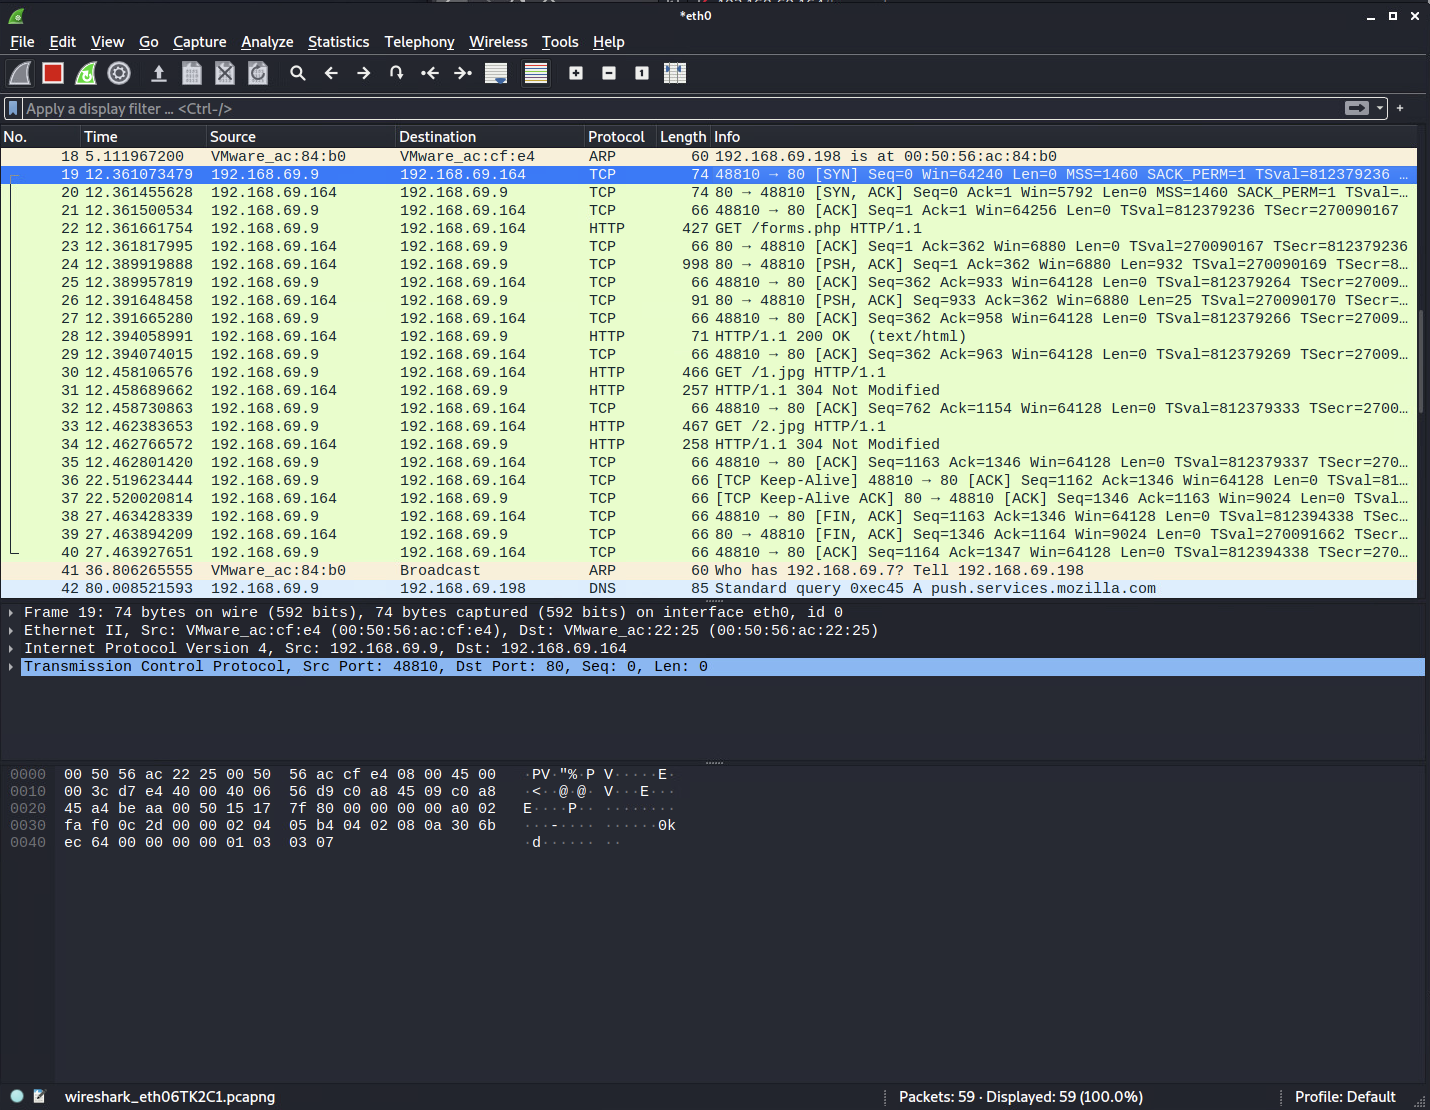
\includegraphics[width=0.8\textwidth]{figures/Wireshark Traffic}
  \caption{Wireshark Traffic}
  \label{f:Wireshark Traffic}
\end{figure}

The browser sets the IP through the TCP protocol and SYN requests are sent
between the two IPs. Since it's TCP there is the handshake with ACK and
SYN-ACK\@. The website content is retrived through HTTP and there are GET
requests that fetch images on root.

\section{Task 4: Enumation of Tables}
\label{task4-database}

With the command below, we are able to get the database name.
\begin{figure}[H]
  \centering
  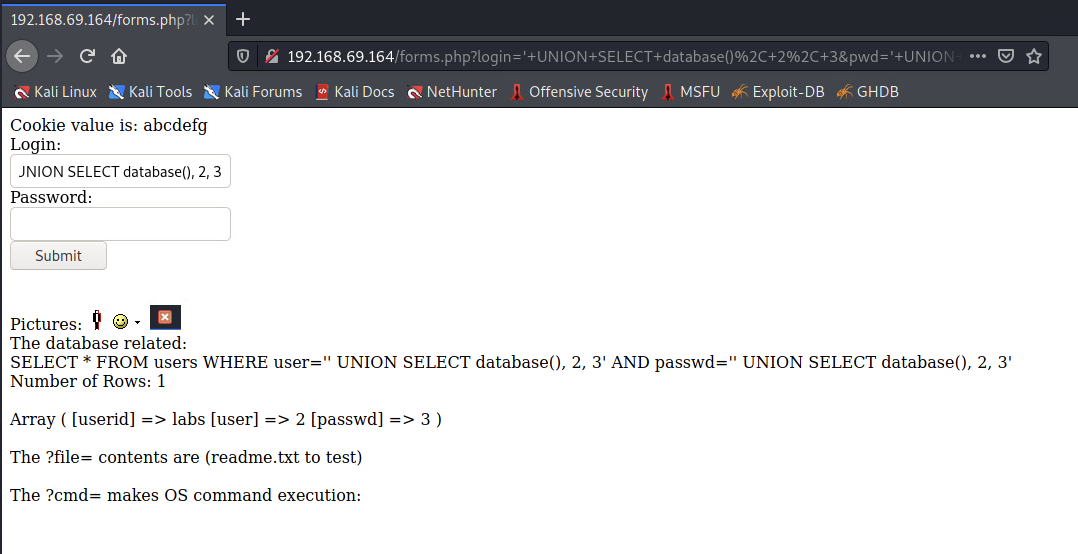
\includegraphics[width=0.8\textwidth]{figures/database_name}
  \caption{Name of Database}
  \label{f:database-name}
\end{figure}

The command below retrieves all the tables in the database.
\begin{figure}[H]
  \centering
  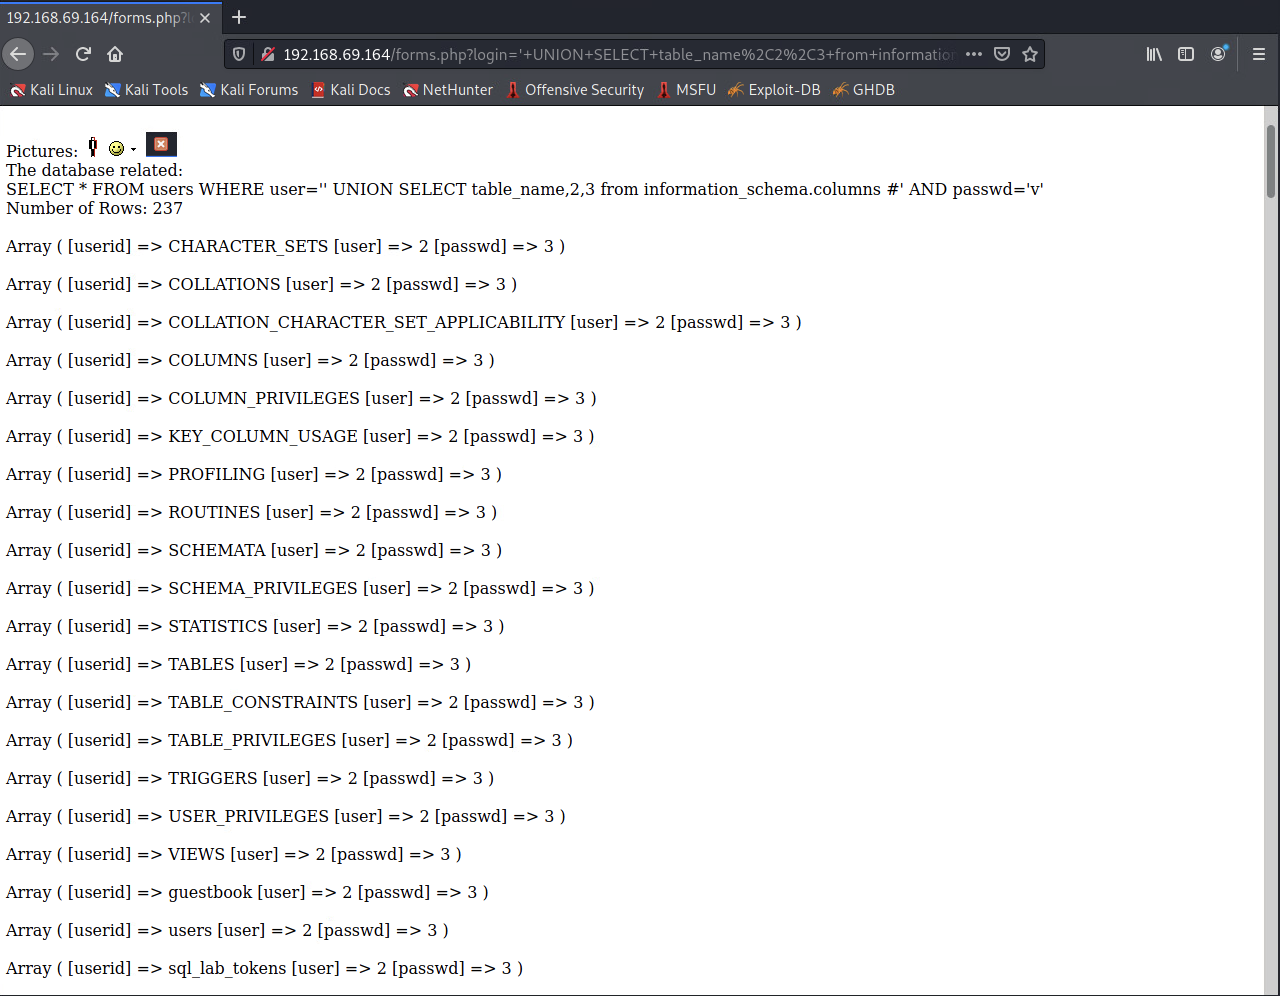
\includegraphics[width=0.8\textwidth]{figures/all_tables}
  \caption{Enumeration of Tables}
  \label{f:all_tables}
\end{figure}

From the information retrieves before, we know that the database we are interested in is labs.
It can be used to filter the query and get the tables names.
\begin{figure}[H]
  \centering
  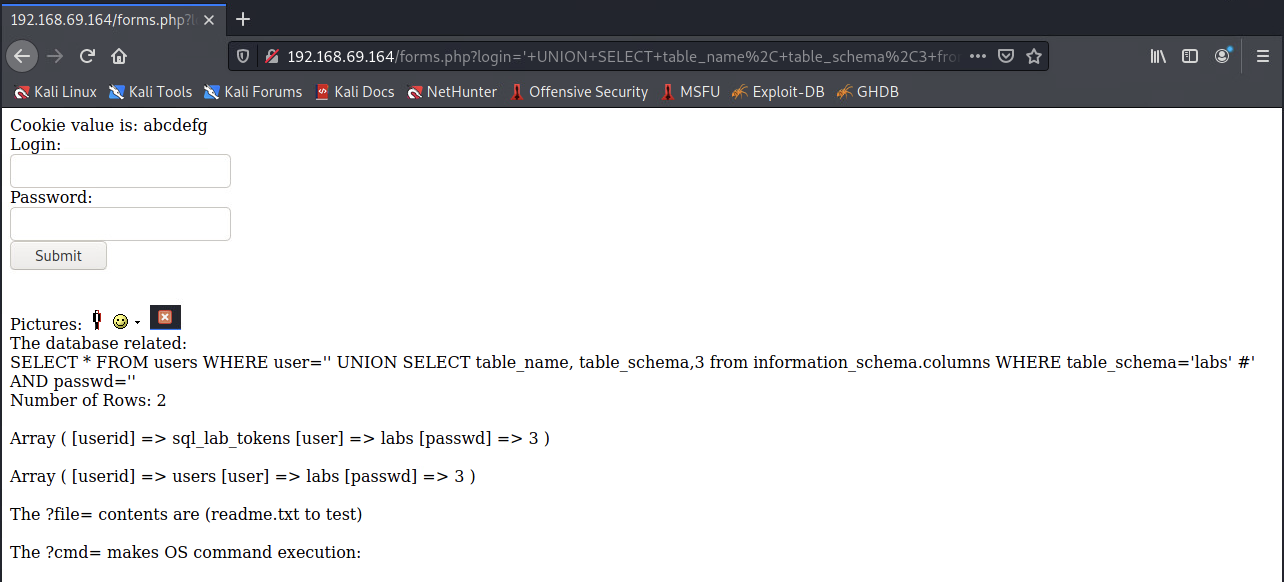
\includegraphics[width=0.8\textwidth]{figures/labs-tables}
  \caption{Labs Tables}
  \label{f:labs-tables}
\end{figure}

With the following query we get the column names.
\begin{figure}[H]
  \centering
  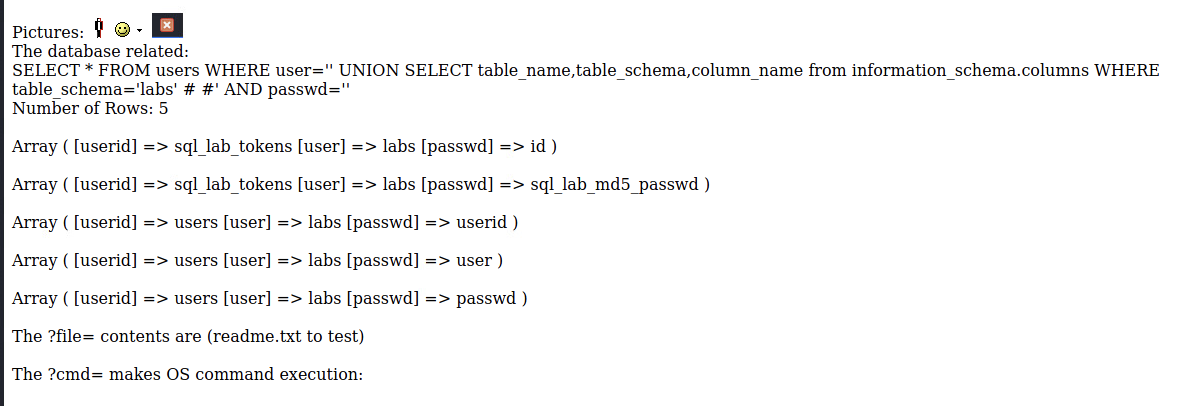
\includegraphics[width=0.8\textwidth]{figures/column-names-labs-table}
  \caption{Column names for Labs table}
  \label{f:column-names-labs-table}
\end{figure}

Since the \ref{s:task6-7-md5-hash-tokens} requires to crack the md5 hashes, we
check for names that reference it.
Once found sql\_lab\_md5, we access it with the following query.
\begin{figure}[H]
  \centering
  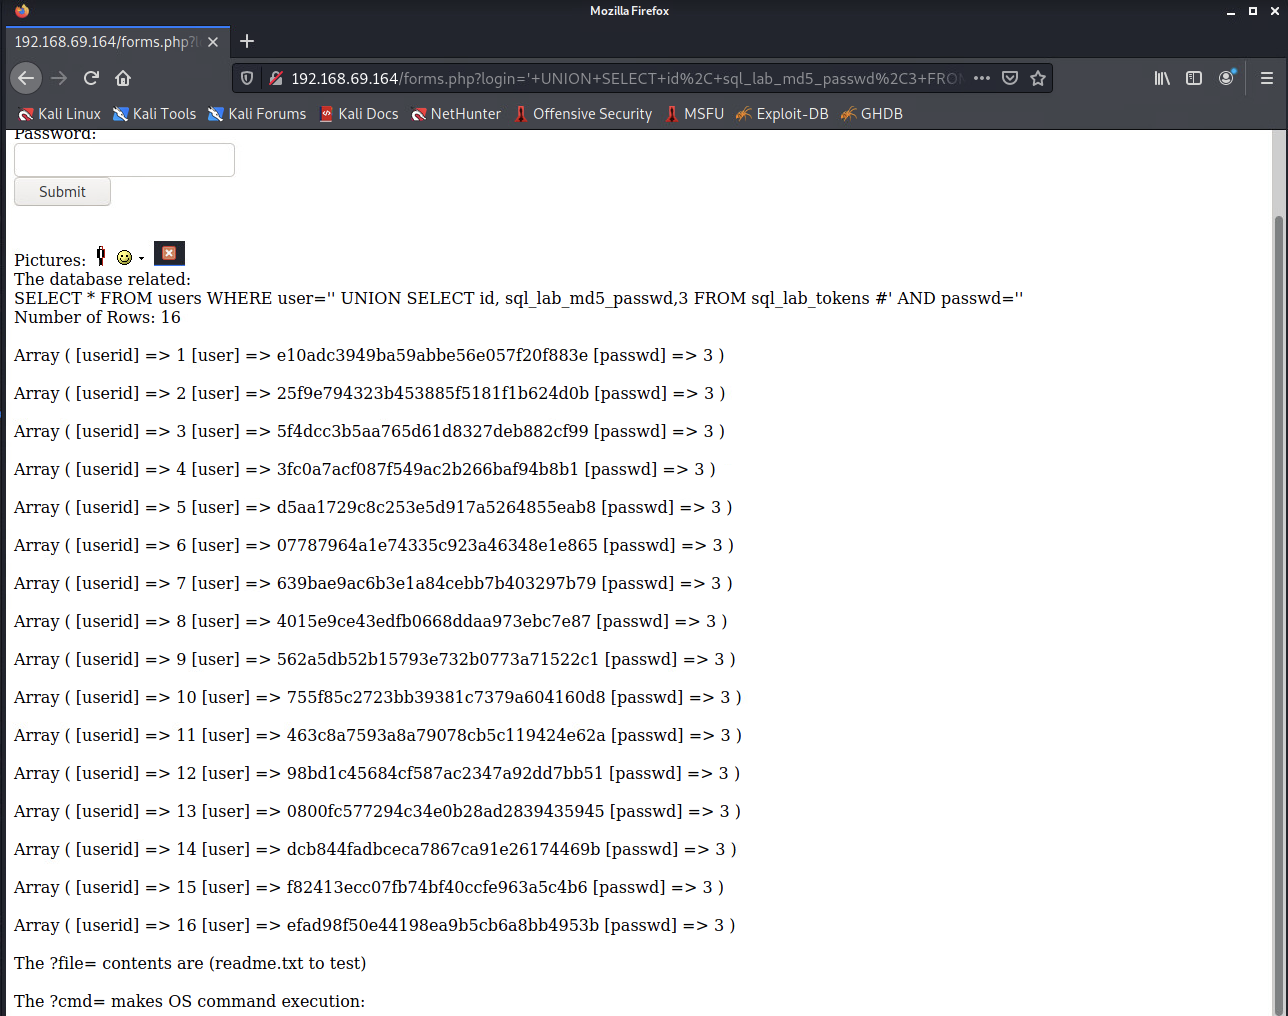
\includegraphics[width=0.6\textwidth]{figures/md5-hashes}
  \caption{MD5 Hashes}
  \label{f:md5-hashes}
\end{figure}

\section{Task 5: Username with userid 4}
\label{task5-username}

\begin{figure}[H]
  \centering
  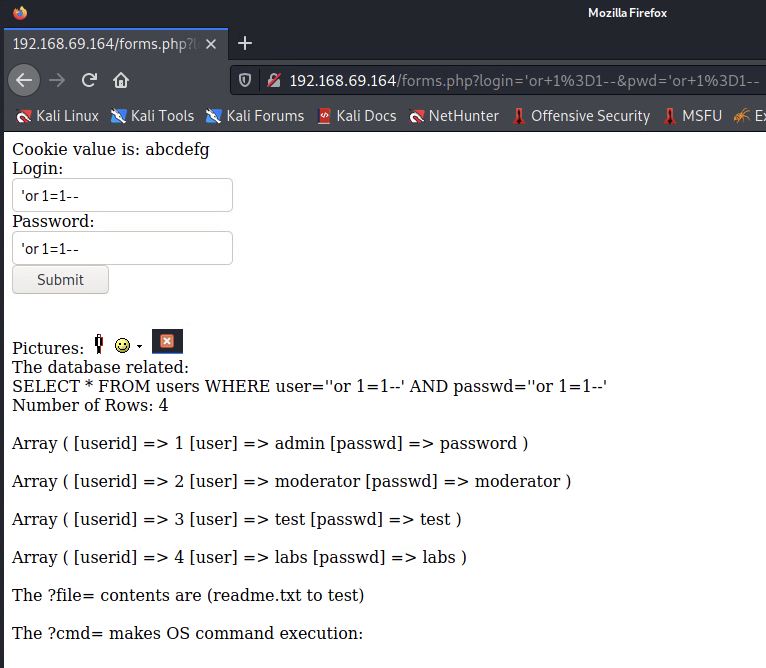
\includegraphics[width=0.6\textwidth]{figures/tables}
  \caption{Username}
  \label{f:username}
\end{figure}

\section{Task 6 \& 7: MD5 Hashes}
\label{s:task6-7-md5-hash-tokens}
The hashes in \ref{f:md5-hashes} are the MD5 hashes that we will manually crack.
I picked two random hashes to crack them on crackstation as specified in the task.
Below a screenshot with the results of the action.

\begin{figure}[H]
  \centering
  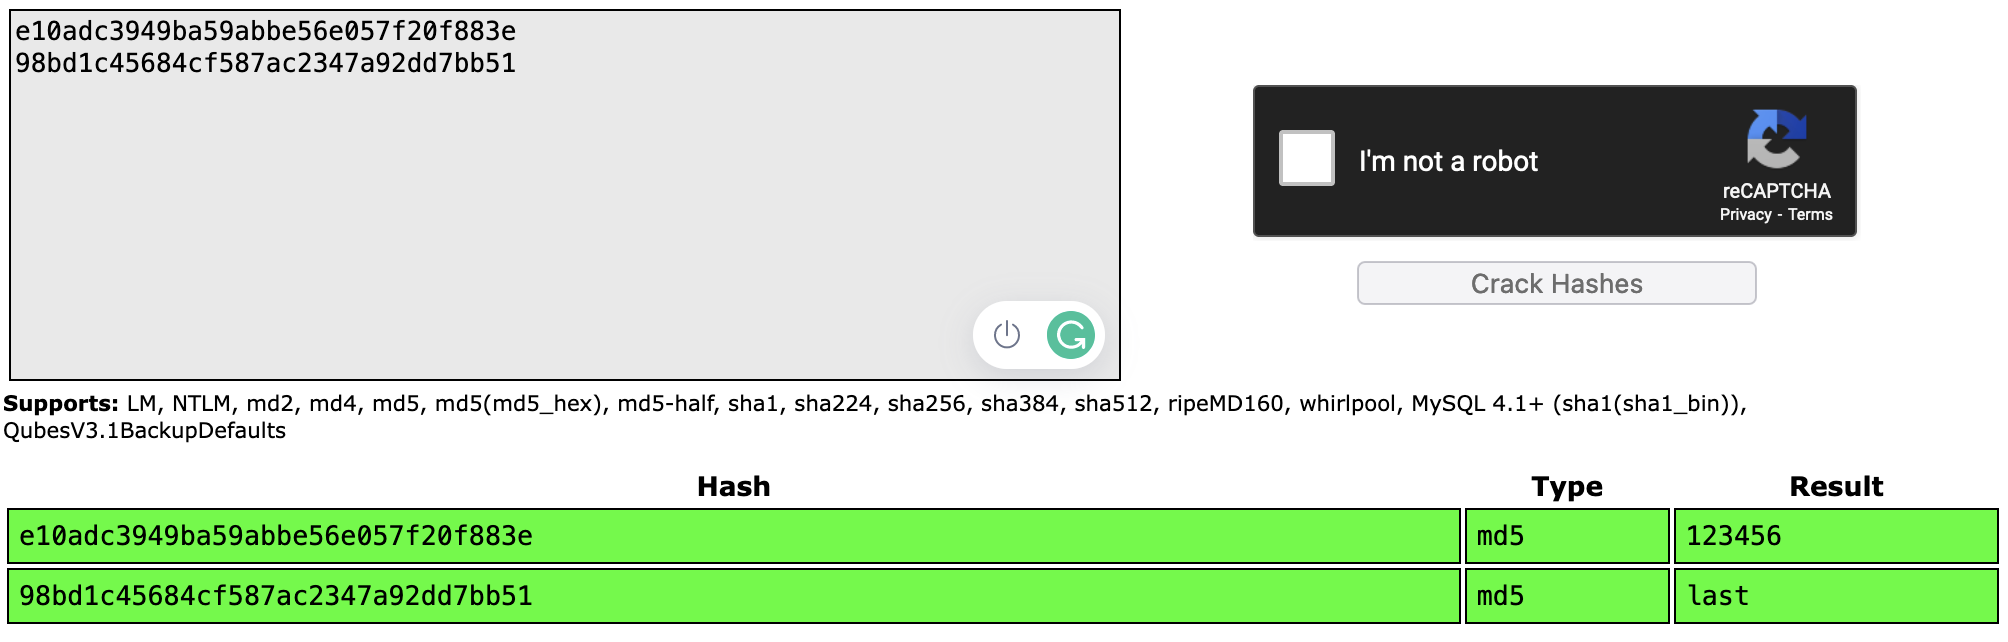
\includegraphics[width=1\textwidth]{figures/crackstation}
  \caption{Crackstation Result}
  \label{f:crackstation}
\end{figure}


\section{Task 8: XSS Demonstration}
\label{task8-xss}
A cross-site scripting attack has been performed on the web service provided.
The editboxes can be used to run malicious JavaScript code.
The code below shows how easy is to inject malicious code into script tags.
\begin{figure}[H]
  \centering
  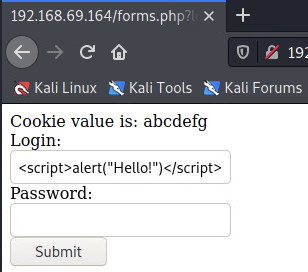
\includegraphics[width=0.5\textwidth]{figures/xss-demonstration}
  \caption{Inject Script Tags}
  \label{f:xss-demonstration}
\end{figure}

Below a proof that the code is execute on the client.

\begin{figure}[H]
  \centering
  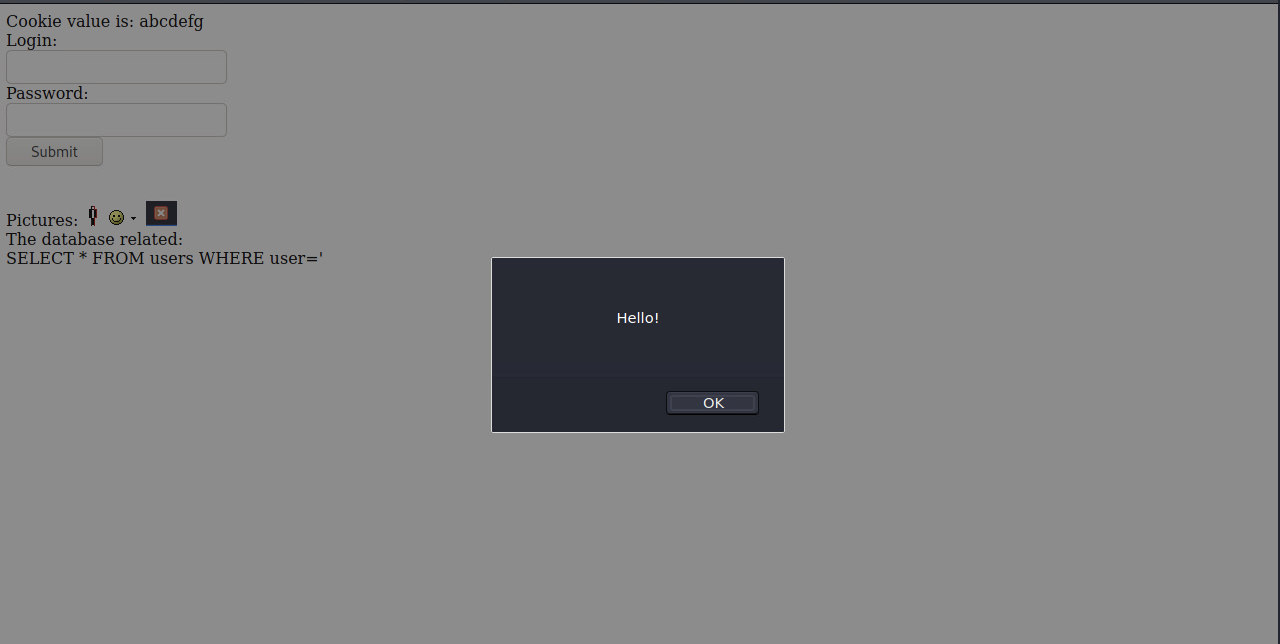
\includegraphics[width=0.6\textwidth]{figures/code-execute}
  \caption{code-execute}
  \label{f:code-execute}
\end{figure}

\section{Task 9: View Files}
\label{task9-view-files}
It is possible to run commands through the LFI vulnerability. In the images below
we can see how we used the browser to access and read files specified in the task.
\begin{figure}[H]
  \centering
  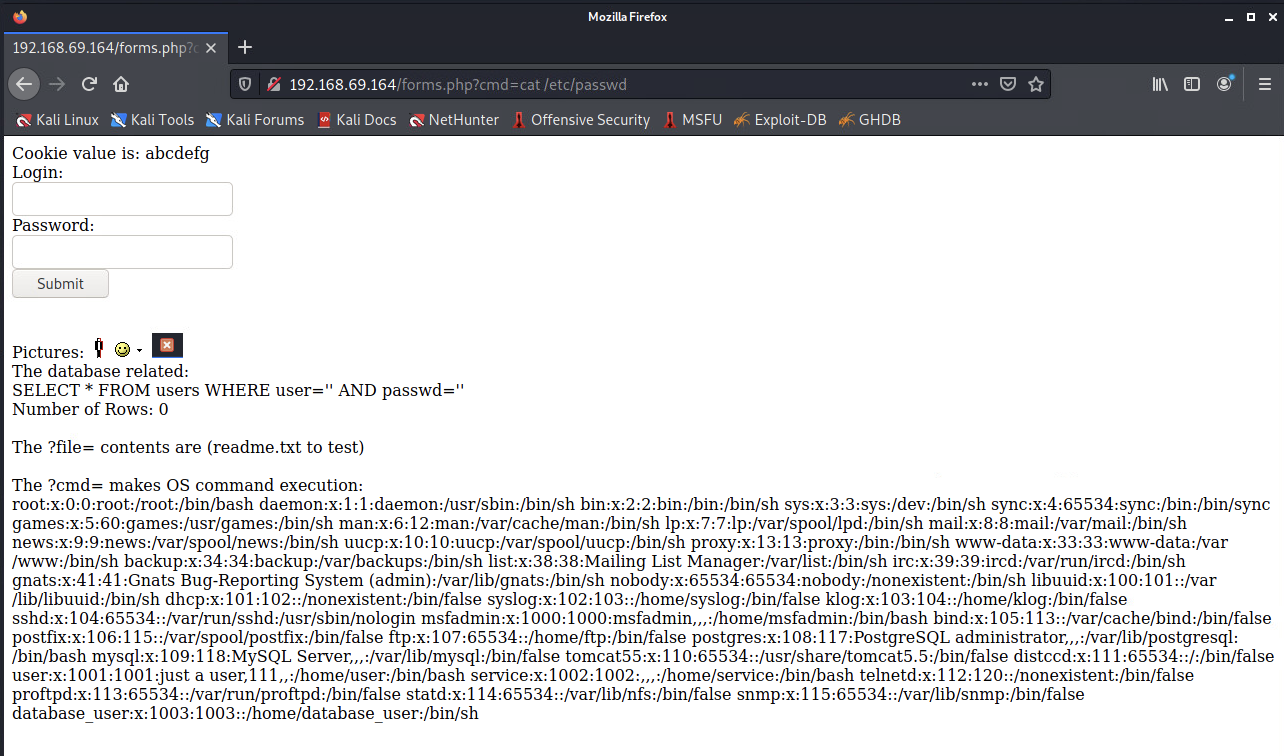
\includegraphics[width=0.6\textwidth]{figures/passwd}
  \caption{LFI: passwd}
  \label{f:passwd}
\end{figure}

In the picture below we view the access logs.
\begin{figure}[H]
  \centering
  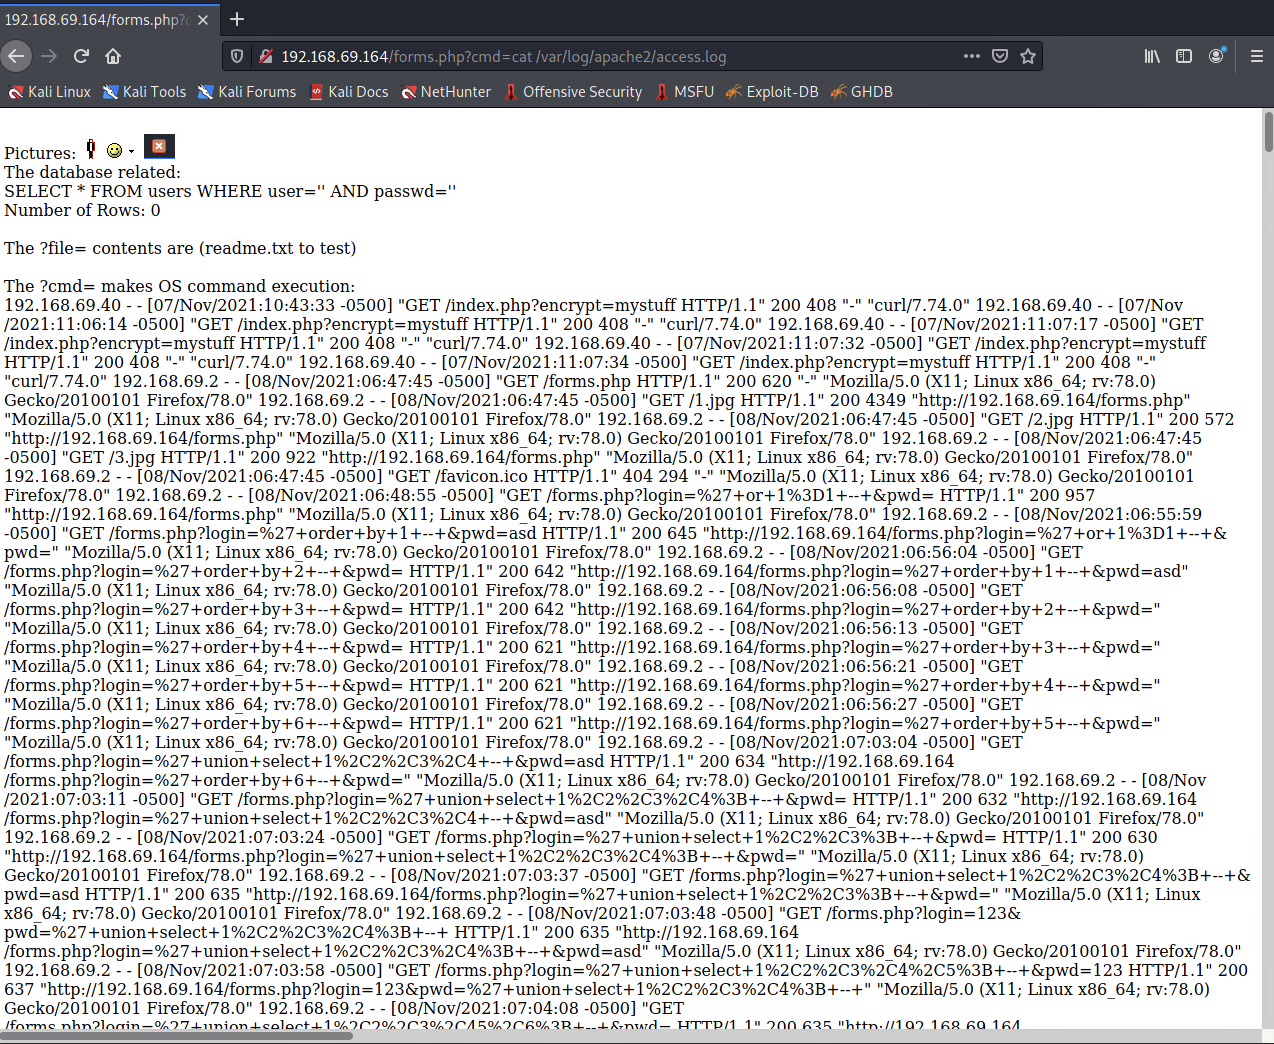
\includegraphics[width=0.8\textwidth]{figures/task9-access-log}
  \caption{LFI: Access Logs}
  \label{f:task9-access-log}
\end{figure}

In the picture below the shadow bak
\begin{figure}[H]
  \centering
  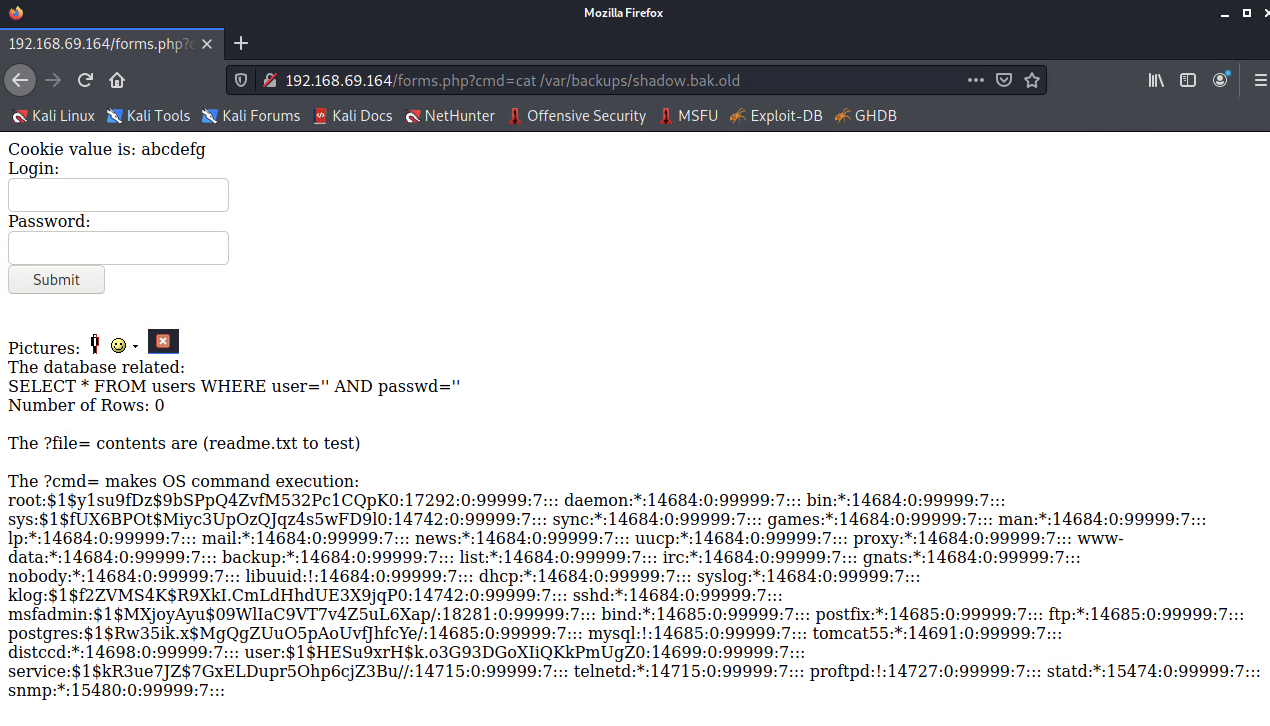
\includegraphics[width=0.8\textwidth]{figures/shadow-bak}
  \caption{LFI: Shadow}
  \label{f:shadow-bak}
\end{figure}

It's worth noting that there are many LFI and bypasses techniques, such as
traversal sequences stripped non-recursively and null byte (for php).
